\apendice{Documentación de usuario}

\section{Introducción}
Esta sección está centrará en el uso que se puede hacer de la aplicación por parte del usuario. Se explicarán las distintas funcionalidades y el uso esperado que se puede hacer de ellas.
\section{Requisitos de usuarios}
Dado que la herramienta desarrollada se trata de una aplicación web y no una aplicación de escritorio el usuario no estará sujeto a estrictos requisitos técnicos que puedan involucrar la compatibilidad de su equipo con la aplicación.

 A continuación se hará un pequeño listado de los requisitos esperados por parte de los usuarios:
 
 \begin{itemize}
 	\item \textbf{Dispositivo}: Ordenador o dispositivo móvil con capacidad de conexión a Internet.
 	\item \textbf{Conexión a Internet}: Dado que la herramienta se trata de una aplicación web es imprescindible contar con conexión a Internet.
 	\item \textbf{Navegador}: Se requiere un navegador actual compatible con HTML5 y CSS3.
 	\item \textbf{JavaScript}: Parte del funcionamiento de la aplicación del lado del cliente depende de JavaScript, por lo que este debe de estar habilitado en el navegador.
 	\item \textbf{Cuenta de usuario}: Algunas de las funcionalidades requieren de contar con una cuenta de usuario, además de haber iniciado sesión.
 \end{itemize}


\section{Instalación}

Salvo que se quiera realizar una ejecución a nivel local de la aplicación no es necesario realizar una instalación, bastando con simplemente acceder a la \href{https://usmt-68ffcbc61e83.herokuapp.com/home}{URL} de la aplicación para poder hacer uso de ella.

En caso de que se quiera instalar localmente, se pueden seguir los pasos descritos en la sección de \hyperref[sec:compilación]{compilación, instalación y ejecución} en el manual del programador.
\section{Manual del usuario}

Para poder acceder a la aplicación bastará con ir a la dirección \url{https://usmt-68ffcbc61e83.herokuapp.com/home} desde nuestro navegador.

La aplicación consta de las siguientes pestañas.

\subsection{Home}

Esta es la pantalla inicial de la aplicación. Esta sirve como simple introducción para el usuario. 

\imagen{USMThome}{Pantalla de inicio de la aplicación web}

En el margen superior de la pantalla se muestra una barra de navegación. A través de esta se podrá acceder a las distintas funcionalidades de la aplicación.

\imagen{USMTnavbar}{Barra de navegación de la aplicación}

Las opciones mostradas se corresponden con lo siguiente:
\begin{itemize}
	\item \textbf{Home}: La pantalla de inicio de la aplicación.
	\item \textbf{Mapas}: Se corresponde con la visualización de las distintas ciudades y sus respectivos establecimientos comerciales. Para poder obtener recomendaciones hay que acceder aquí.
	\item \textbf{Visualización de red}: Visualización de la interacción entre las categorías comerciales de las distintas ciudades en forma de grafo. Contiene funcionalidades para seleccionar ciudad y filtrar en base a grado y grupo.
	\item \textbf{Usuarios}: En la esquina superior derecha se dispone un menú desplegable para las funcionalidades de usuarios. Son las siguientes:
	\begin{itemize}
		\item \textbf{Iniciar Sesión}
		\item \textbf{Registrarse}
		\item \textbf{Cerrar Sesión}
	\end{itemize}
\end{itemize}

\subsubsection{Usuario}

Para acceder las funcionalidades de recomendaciones será necesario contar con una cuenta e iniciar sesión.

Para ello contamos con el menú desplegable de la esquina superior derecha.
\begin{figure}[h!]
	\centering
	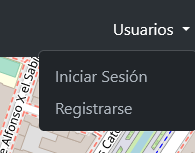
\includegraphics[scale=0.4]{USMTdesplegableusuarios}\\
	\caption{Desplegable de usuarios}
\end{figure}


\subsubsection{Visualización de red}

Una de las funcionalidades de la aplicación es ver la interacción entre las distintas categorías de cada ciudad en formato de grafo. Se ha provisto con una visualización interactiva que permite aplicar distintos efectos.

Al acceder a ella nos encontraremos con lo siguiente:

\imagen{USMTvisred1}{Visualización inicial red de categorías}

Como podemos ver se encuentra vacía. Para poder visualizar el grafo tendremos que seleccionar una ciudad del menú desplegable con nombre <<Ciudades>> en el lado derecho de la pantalla.

\imagen{USMTvisred2}{Visualización de red de ciudad}

Tardará unos segundos en mostrarnos la visualización, se nos indicará con un icono circular. Una vez cargada la visualización se nos aparecerá un grafo, teniendo los nodos una etiqueta que les asocia a la categoría a la que representan. Si situamos el cursos sobre ellos se nos mostrará el número de ubicaciones con dicha categoría que la ciudad seleccionada posee. En el caso de los enlaces se nos indicará el número de veces que las categorías enlazadas interactúan entre sí por proximidad. En cuanto al código de colores los nodos amarillos son aquellos asociados a servicios y los azules a tiendas. La visualización también posee físicas, por lo que se puede arrastrar los nodos y ver cómo responden.

Otra de las opciones que posee el menú lateral es el del filtro por grado. Esta reducirá el número de nodos en base al grado de estos. Está implementado usando un \textit{slider}, pudiéndolo deslizar para filtrar fácilmente. Esto es de especial utilidad si buscamos encontrar un núcleo reducido de las categorías más importantes de la ciudad.

\imagen{USMTvisred3}{Visualización de la red con filtro de grado}

La última opción de la que disponemos es el filtro por grupo. Dado que la red está compuesta por dos grupos, tiendas y servicios; es interesante poder visualizar únicamente uno de ellos. Además puede aplicarse con el filtro de grado, pudiendo obtener las categorías más importantes de ambos grupos.

\imagen{USMTvisred4}{Visualización de la red con filtro de grupo}

\subsection{Mapas y recomendaciones}

Otra de las funcionalidades de la aplicación es la visualización de los establecimientos comerciales de las ciudades. Primero tendremos que acceder a la opción <<Mapas>> de la barra de navegación. En esta tendremos que seleccionar la ciudad y la categoría que buscamos en el menú de la parte derecha de la pantalla. Una vez hecho pulsaremos sobre <<Buscar>>

\imagen{USMTmapassearch}{Menú de búsqueda de visualización de mapas}

Al pulsar sobre el botón el mapa se moverá hacia la ciudad seleccionada y visualizará los marcadores con los establecimientos comerciales de la categoría seleccionada. Podemos pasar el cursor sobre ellos y se nos mostrará alguna información del lugar.

\imagen{USMTmarkerinfo}{Información de marcador}

Para poder realizar las recomendaciones sobre los lugares que estemos interesados tendremos que hacer \textit{click} sobre sus marcadores. Estos pasarán a ser de color rojo. Si queremos deseleccionarles podemos volver a hacer \textit{click} y volverán a su estado normal. Podemos seleccionar múltiples de ellos.

\imagen{USMTselectedmarkers}{Marcadores de establecimientos seleccionados}

Puede que también estemos interesados en lugares que no están registrados en la aplicación solo en base a su ubicación y no en base a su categoría. Para hacer esto simplemente podemos hacer \textit{click} en cualquier sitio del mapa y aparecerá un marcador de color verde, para diferenciar de las ubicaciones registradas. Pueden coexistir con los marcadores de establecimientos reales y tienen un funcionamiento similar a estos.

\imagen{USMTcoordsmarkers}{Marcadores de coordenadas seleccionadas}

Al buscar nuevamente establecimientos de otra categoría comercial teniendo ya seleccionados algunos estos se mantendrán junto con las coordenadas seleccionadas.

Si deseamos eliminar todos los marcadores seleccionados podemos usar el botón de <<Borrar>> que los eliminará del mapa.